\documentclass[a4paper]{article}

\usepackage[english]{babel}
\usepackage[utf8]{inputenc}
\usepackage{amsmath}
\usepackage{graphicx}
\usepackage[colorinlistoftodos]{todonotes}
\usepackage{float}
\usepackage{url}

\title{Screens on Screen on Screens - The Multiple Computer Monitor Setup}

\author{Matthew W. Flickner}

\date{\today}

\begin{document}
\maketitle

\begin{abstract}
Through the analysis of previous studies, usability metrics from Interaction Design, and cognitive psychology, the analysis of a multiple monitor computer setup opposed to a single monitor setup shows that computers set up to use two monitors opposed to one is far more effective and efficient for the user. This is due primarily to visual processing of the brain and increased window visibility. While not yet perfect, this study concludes that a dual monitor setup is a far better alternative than a single monitor on a computer.
\end{abstract}

\section{Introduction}
In Dave Eggers' \emph{The Circle}\/, Mae Holland works at a power tech company called the Circle. She starts off at low position but quickly rises through the ranks at the company. Each time she is promoted, she is given a new computer monitor to perform her new tasks on. Eventually her workspace is covered with monitors. The Circle tries to maximize Mae's efficiency by dividing her tasks and duties by computer monitor \cite{EggersCircle}. This brings about the discussion as to whether a single monitor is more or less effective than multiple monitors. And at what point, if any, does a computer user have too many monitors and lose effectiveness? The efficiency, effectiveness, and satisfaction of a single monitor setup opposed to a multiple monitor setup will be explored through the rest of the paper through the analysis of previous works, effectiveness and usability strategies, and psychological analysis.

\section{Background/Prior Work}
\subsection{Origin of the Multiple Monitor}
While the computer monitor has been an essential part of the modern computer for some time, computers utilizing multiple monitors have been more recently developed in the past twenty years. The ability of computers to be able to support multiple monitors has been for around since 1998 on Windows systems and 22 years on the Macintosh system \cite{Grudin}. Since then, technology has evolved to allow numerous monitors to connect to a single computer.
% JD: Citations should go before the period.  (I changed it here but to save time
%     won't change future instances)

\subsection{Prior Work}
Since the introduction of technology allowing computers to support multiple monitor, researchers have conducted many usability studies studying the efficiency, learnability, and effectiveness comparing users using multiple monitors with users with a singular monitor.

\subsubsection{Grudin's Study}
Jonathan Grudin's study compared the multiple monitor setup upgrade with a larger monitor upgrade and was a huge supporter of the multiple monitor set up. He compared using multiple monitors with a single large monitor to having a house with one large room or with multiple rooms. One could theoretically have a house with one large room that can be used for all purposes. In that one-roomed house there could be everything a person needs to get by. There could be a kitchen, a living room, a work study, and a bed. But it would be far more convenient according to Grudin to have the house with multiple rooms, with each room serving a particular purpose \cite{Grudin}. Grudin's experiment of testing multiple monitors against a single monitor yielded several important observations. Grudin observed that users using a second monitor did not use it as additional space by straddling a window across the two monitors \cite{Grudin}. Grudin also observed that one monitor became the ``primary monitor'' and was used for the main task while the second monitor was used primarily for secondary tasks to support the primary task.
% JD: Nice find, this study.

\subsubsection{Truemper's Study}
This study took a lot of what Grudin did and expanded on it. In addition one important observation that came with this study was the usage of more than just two monitors. The study used four monitors and discover that the amount of time spent using just two monitors was far greater than the time using three monitors which was far greater than the time spent using four monitors \cite{Truemper}. This suggested that a certain amount of monitors could potentially be unnecessary for users.
\begin{figure}[H]
\centering
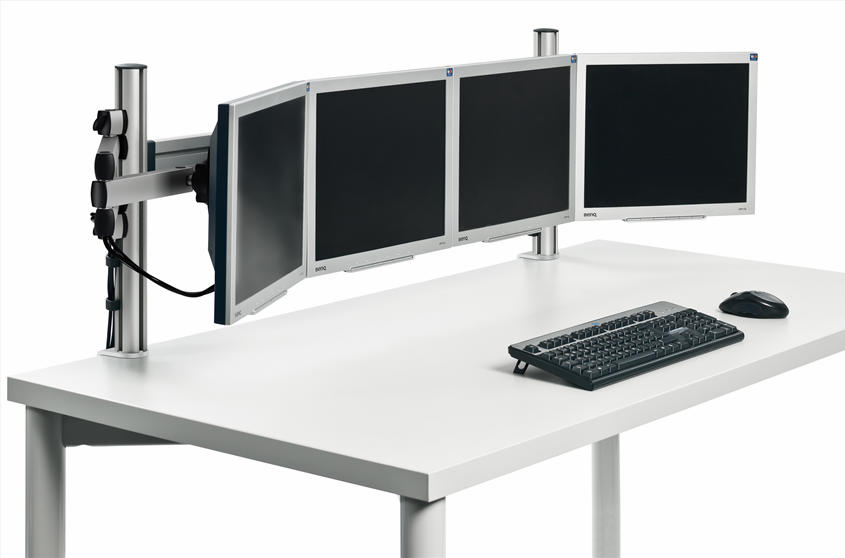
\includegraphics[width=0.8\textwidth]{4inRow.jpg}
\end{figure}
% JD: Another good-sounding one, though I think its coverage could have been
%     better.  The mixing of monitors and windows in the last sentence is not
%     perfectly clear to me and more explanation would have been nice.

\subsection{Previously Established Positives of Multiple Monitors}

\subsubsection{Window Visibility}
The multiple monitor setup created a larger average window visibility \cite{Hutchings}. This lessened the need for window minimization and maximization with users \cite{Grudin}. With a larger working space users could spread out their windows to work more comfortably \cite{Truemper}. However the average window number of windows' visibility was not significantly larger than users with single monitors although this is mostly attributed to multiple monitor users using much larger sized windows \cite{Hutchings}.

\subsubsection{Improved Efficiency of Tasks}
Multiple monitors for one thing definitely improve the efficiency of their users. Users with multiple monitors had better productivity due to lower task completion time and workload \cite{Kang}.

\subsubsection{Bezels}
Bezels are areas between screens \cite{Truemper}. Basically they are the borders of a screen on an individual monitor. When screens are put together in a multiple monitor setup, bezels are useful for supporting multitasking and separating windows with different tasks.



\subsection{Previously Established Negatives of Multiple Monitors}

\subsubsection{Distance to Travel}
With multiple monitors, the distance to travel across the screen is a large factor. Truemper cites the issue of when using the Windows operating system, the user must travel a further distance to reach the start menu in the bottom left corner \cite{Truemper}. This has since been resolved with a keyboard button that brings up the start menu when pushed. However the overall issue of distance to travel is still a issue for other more general scenarios \cite{Truemper}. In addition, further distance to travel usually calls for a higher mouse tracking velocity which makes it easier to lose the mouse on the screen \cite{Truemper}.

\subsubsection{Bezels}
Bezels have a negative side to them as well. They create a visual discontinuity.  When a cursor crosses the path of a bezel, its path is often deflected.
\begin{figure}[H]
\centering

\includegraphics[width=0.8\textwidth]{bezel-example.jpg}
\caption{Classic example of bezel visual discontinuity}
\end{figure}
It is possible to calibrate monitors to avoid this issue but the issue then is still a gap between pixels where the bezels exist \cite{Truemper}.

\subsubsection{Too Many Monitors}
Studies have shown that after a certain amount of screens, some screens are barely used. Truemper's study used four monitors and the amount of time spent using all four monitors was less than two percent of the time \cite{Truemper}.
\begin{figure}[H]
\centering
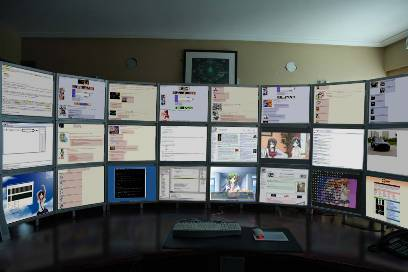
\includegraphics[width=0.8\textwidth]{so-many.jpg}
\end{figure}
% JD: Aha---so they *were* all about monitors.  When you first talked about this study
%     the terms "monitor" and "window" got mixed up.

\subsubsection{Lack of Application Support}
Many applications do not optimize their software to be used efficiently with a multiple monitor setup \cite{Grudin}. Often times application open on a different screen than the screen the user intended them to \cite{Grudin}.


\section{Method}
The prevailing option at the moment is that a multiple monitor setup is more efficient and productive than a single monitor setup. Because of this, multiple monitor setups are becoming more and more prevalent in work environments and will continue to become more of a norm. The studies of Grudin, Truemper, Kang, and Hutchings are all very relevant studies on the topic and separated by a few years which gives good insight into how usability in multiple monitors has changed as technology has improved over the years. Grudin's study is the basis for many studies to follow and Truemper and Kang are more recent studies. I will use the positive and negative results of a multiple monitor setup from previous works and usability concepts discussed in class along with the psychology of laterality presented by Dr. Hellige to analyze the effectiveness of multiple monitors, singular monitors, and monitor size and draw a conclusion on the most effective way to utilize a computer monitor system.

\section{Discussion}
\subsection{Window Visibility, Improved Efficiency, and Bezels - Why the Positives are Positives}
Window visibility is a huge positive of a multiple monitor setup. One could have several windows open on each screen, reducing the need for minimization and maximization of windows and making these windows quickly accessible. Minimization and maximization are a big deal when it comes to Fitt's Law because of the distance the mouse must travel to minimize and maximize the windows at the top corner of the window for minimization and the bottom of the screen for maximization unless the user knows keyboard shortcuts to achieve this \cite{Tog}.
\subsubsection{The Windows OS Window-Snap Feature}
The single monitor setup has become more efficient recently with the addition of the window-snap feature in Windows 7 and above. The feature allows the user to drag a window into either the left side or right size of the screen and the window will auto-resize to fill half of the screen. This feature greatly increases user efficiency on a single monitor setup running Windows because it basically allows a single screen to act as two by easily allowing the user to split it in half. However a user running Windows in a dual monitor screen could also utilize this feature, except use it on both his monitors.
\subsubsection{The Psychological Edge}
Psychologically, the dual monitor case, especially in the case of two monitors side by side, is a more effective setup. Since the visual processing of the brain, sends one visual field to one side of the brain and the other visual field to the other, thanks to the corpus callosum, a setup of two monitors could allow one side of the brain to process one screen and the other side of the brain to process the other. Since the corpus callosum allows the two sides of the brain to communicate with one another, this would lead to an improved efficiency of tasks as the brain could already theoretically be processing the visual field as the user moves their attention towards it. The bezel then is simply a divider of the two visual processing fields.

\subsection{Distance Traveled, Bezels, Lack of Application Support, and Monitor Overload- Why the Negatives are Negatives and Possible Solutions}
Distance to travel is an issue because of Fitts's law. The mouse traveling further distances takes more time and more motion of the hand \cite{Tog}. Faster tracking mice is one way to solve this problem but it then becomes easier to lose the mouse. A solution to this is visually denser mice, which are easier for the eye to track, even at high speeds \cite{Truemper}. In a single monitor setup, distance to travel factors as well. Since a single monitor setup does not have as much window visibility, the distance to travel factors in with the minimizing and maximizing of more windows. So distance to travel has a negative effect in both a multiple monitor setup and a single monitor setup. Bezels are only negative when trying to expand a single window over multiple screens. But users tend to not do this and rather use the two screens for separate tasks \cite{Grudin}. Lack of application support falls onto the designers of the application, they must make it so their applications are more efficient and effective with supporting multiple monitors.
\begin{figure}[H]
\centering
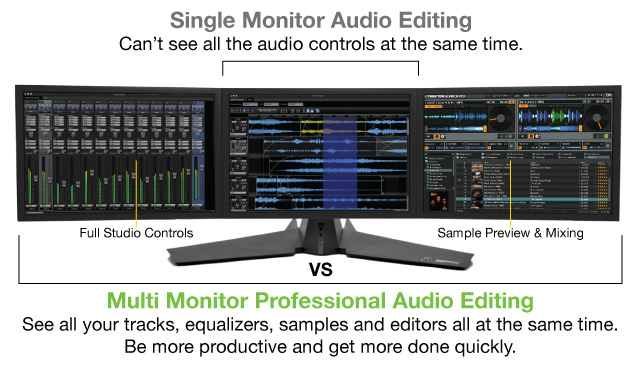
\includegraphics[width=0.8\textwidth]{application-optimization.jpg}
\caption{Application that has successfully been optimized for a multiple monitor setup.}
\end{figure}
The developers need to figure out how to make applications show up on the right monitor when opened make sure they going with the flow of where the user intuitively thinks something with show up \cite{Grudin}. The only real issue other than distance traveled is the possible monitor overload. When more monitors are added to a user's work environment, some of the additional screens are barely used. A fourth screen was found to only be used less than two percent of the time.\cite{Truemper}

\subsubsection{The Psychological Reasoning Behind Monitor Overload}
Psychologically, the reasoning behind why monitor overload occurs is very similar to the reasoning as to why a dual monitor setup is very effective. Since the brain produces only a left visual field and a right visual field, adding more than two monitors would psychologically make the brain less efficient at processing visually what is in front of it. Whether the extra monitor (or monitors) is on the left, right, top, or bottom of the first two, it adds one more visual object for the occipital lobe to process.
% JD: Hmmmm...this is a bit of a stretch.  But I appreciate the game effort
%     to integrate Dr. Hellige's talk.

\subsection{Satisfaction}
Perhaps the most important show of superiority in the dual monitor setup is user satisfaction. User satisfaction is one of the most important usability metrics. If the user is satisfied then whatever they are using is doing a lot right \cite{Nielsen}. Users in studies reported says ``I would not go back'' and ``Without it, I feel very limited'' \cite{Grudin}. In addition users said that the dual monitor system "had spoiled them" \cite{Grudin}. When users are satisfied, it tends to mean that whatever they are satisfied about works better than what they are used to \cite{Nielsen}. In this case it is satisfaction of a multiple monitor setup being more effective than their standard single monitor setup.

\section{Conclusion}
The multiple monitor setup clearly has the edge over a single monitor setup in today's computer world. It's boosting of window visibility and user efficiency make it a far better setup than a single monitor. 
\begin{figure}[H]
\centering
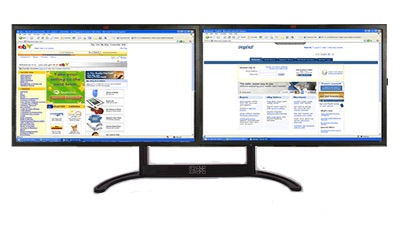
\includegraphics[width=0.8\textwidth]{two-monitors.jpg}
\caption{Application that has successfully been optimized for a multiple monitor setup.}
\end{figure}
Plus many of the negatives in a dual monitor setup also are present in a single monitor situation. In addition, users are far more satisfied with their experience using two monitors. And psychologically, it makes sense. With our two visual processing fields being processed by different sides of the brain and then linked by the corpus callosum, a dual monitor setup is ideal as it allows for one monitor to be visually processed by each side of the brain. Two monitors, by far, makes a more efficient, effective, and satisfied user.

\bibliography{references}
\bibliographystyle{plain}
\end{document}